\documentclass[]{article}
\usepackage{lmodern}
\usepackage{amssymb,amsmath}
\usepackage{ifxetex,ifluatex}
\usepackage{fixltx2e} % provides \textsubscript
\ifnum 0\ifxetex 1\fi\ifluatex 1\fi=0 % if pdftex
  \usepackage[T1]{fontenc}
  \usepackage[utf8]{inputenc}
\else % if luatex or xelatex
  \ifxetex
    \usepackage{mathspec}
  \else
    \usepackage{fontspec}
  \fi
  \defaultfontfeatures{Ligatures=TeX,Scale=MatchLowercase}
\fi
% use upquote if available, for straight quotes in verbatim environments
\IfFileExists{upquote.sty}{\usepackage{upquote}}{}
% use microtype if available
\IfFileExists{microtype.sty}{%
\usepackage{microtype}
\UseMicrotypeSet[protrusion]{basicmath} % disable protrusion for tt fonts
}{}
\usepackage[margin=1in]{geometry}
\usepackage{hyperref}
\hypersetup{unicode=true,
            pdftitle={Mini Proyecto 2020. Datos Tráfico},
            pdfauthor={Stefan Lahud García, Olivia Sarahì Vargas Vásquez},
            pdfborder={0 0 0},
            breaklinks=true}
\urlstyle{same}  % don't use monospace font for urls
\usepackage{color}
\usepackage{fancyvrb}
\newcommand{\VerbBar}{|}
\newcommand{\VERB}{\Verb[commandchars=\\\{\}]}
\DefineVerbatimEnvironment{Highlighting}{Verbatim}{commandchars=\\\{\}}
% Add ',fontsize=\small' for more characters per line
\usepackage{framed}
\definecolor{shadecolor}{RGB}{248,248,248}
\newenvironment{Shaded}{\begin{snugshade}}{\end{snugshade}}
\newcommand{\KeywordTok}[1]{\textcolor[rgb]{0.13,0.29,0.53}{\textbf{{#1}}}}
\newcommand{\DataTypeTok}[1]{\textcolor[rgb]{0.13,0.29,0.53}{{#1}}}
\newcommand{\DecValTok}[1]{\textcolor[rgb]{0.00,0.00,0.81}{{#1}}}
\newcommand{\BaseNTok}[1]{\textcolor[rgb]{0.00,0.00,0.81}{{#1}}}
\newcommand{\FloatTok}[1]{\textcolor[rgb]{0.00,0.00,0.81}{{#1}}}
\newcommand{\ConstantTok}[1]{\textcolor[rgb]{0.00,0.00,0.00}{{#1}}}
\newcommand{\CharTok}[1]{\textcolor[rgb]{0.31,0.60,0.02}{{#1}}}
\newcommand{\SpecialCharTok}[1]{\textcolor[rgb]{0.00,0.00,0.00}{{#1}}}
\newcommand{\StringTok}[1]{\textcolor[rgb]{0.31,0.60,0.02}{{#1}}}
\newcommand{\VerbatimStringTok}[1]{\textcolor[rgb]{0.31,0.60,0.02}{{#1}}}
\newcommand{\SpecialStringTok}[1]{\textcolor[rgb]{0.31,0.60,0.02}{{#1}}}
\newcommand{\ImportTok}[1]{{#1}}
\newcommand{\CommentTok}[1]{\textcolor[rgb]{0.56,0.35,0.01}{\textit{{#1}}}}
\newcommand{\DocumentationTok}[1]{\textcolor[rgb]{0.56,0.35,0.01}{\textbf{\textit{{#1}}}}}
\newcommand{\AnnotationTok}[1]{\textcolor[rgb]{0.56,0.35,0.01}{\textbf{\textit{{#1}}}}}
\newcommand{\CommentVarTok}[1]{\textcolor[rgb]{0.56,0.35,0.01}{\textbf{\textit{{#1}}}}}
\newcommand{\OtherTok}[1]{\textcolor[rgb]{0.56,0.35,0.01}{{#1}}}
\newcommand{\FunctionTok}[1]{\textcolor[rgb]{0.00,0.00,0.00}{{#1}}}
\newcommand{\VariableTok}[1]{\textcolor[rgb]{0.00,0.00,0.00}{{#1}}}
\newcommand{\ControlFlowTok}[1]{\textcolor[rgb]{0.13,0.29,0.53}{\textbf{{#1}}}}
\newcommand{\OperatorTok}[1]{\textcolor[rgb]{0.81,0.36,0.00}{\textbf{{#1}}}}
\newcommand{\BuiltInTok}[1]{{#1}}
\newcommand{\ExtensionTok}[1]{{#1}}
\newcommand{\PreprocessorTok}[1]{\textcolor[rgb]{0.56,0.35,0.01}{\textit{{#1}}}}
\newcommand{\AttributeTok}[1]{\textcolor[rgb]{0.77,0.63,0.00}{{#1}}}
\newcommand{\RegionMarkerTok}[1]{{#1}}
\newcommand{\InformationTok}[1]{\textcolor[rgb]{0.56,0.35,0.01}{\textbf{\textit{{#1}}}}}
\newcommand{\WarningTok}[1]{\textcolor[rgb]{0.56,0.35,0.01}{\textbf{\textit{{#1}}}}}
\newcommand{\AlertTok}[1]{\textcolor[rgb]{0.94,0.16,0.16}{{#1}}}
\newcommand{\ErrorTok}[1]{\textcolor[rgb]{0.64,0.00,0.00}{\textbf{{#1}}}}
\newcommand{\NormalTok}[1]{{#1}}
\usepackage{longtable,booktabs}
\usepackage{graphicx,grffile}
\makeatletter
\def\maxwidth{\ifdim\Gin@nat@width>\linewidth\linewidth\else\Gin@nat@width\fi}
\def\maxheight{\ifdim\Gin@nat@height>\textheight\textheight\else\Gin@nat@height\fi}
\makeatother
% Scale images if necessary, so that they will not overflow the page
% margins by default, and it is still possible to overwrite the defaults
% using explicit options in \includegraphics[width, height, ...]{}
\setkeys{Gin}{width=\maxwidth,height=\maxheight,keepaspectratio}
\IfFileExists{parskip.sty}{%
\usepackage{parskip}
}{% else
\setlength{\parindent}{0pt}
\setlength{\parskip}{6pt plus 2pt minus 1pt}
}
\setlength{\emergencystretch}{3em}  % prevent overfull lines
\providecommand{\tightlist}{%
  \setlength{\itemsep}{0pt}\setlength{\parskip}{0pt}}
\setcounter{secnumdepth}{0}
% Redefines (sub)paragraphs to behave more like sections
\ifx\paragraph\undefined\else
\let\oldparagraph\paragraph
\renewcommand{\paragraph}[1]{\oldparagraph{#1}\mbox{}}
\fi
\ifx\subparagraph\undefined\else
\let\oldsubparagraph\subparagraph
\renewcommand{\subparagraph}[1]{\oldsubparagraph{#1}\mbox{}}
\fi

%%% Use protect on footnotes to avoid problems with footnotes in titles
\let\rmarkdownfootnote\footnote%
\def\footnote{\protect\rmarkdownfootnote}

%%% Change title format to be more compact
\usepackage{titling}

% Create subtitle command for use in maketitle
\providecommand{\subtitle}[1]{
  \posttitle{
    \begin{center}\large#1\end{center}
    }
}

\setlength{\droptitle}{-2em}

  \title{Mini Proyecto 2020. Datos Tráfico}
    \pretitle{\vspace{\droptitle}\centering\huge}
  \posttitle{\par}
  \subtitle{Tratamiento de Datos, Grado en Ciencia de Datos - UV}
  \author{Stefan Lahud García, Olivia Sarahì Vargas Vásquez}
    \preauthor{\centering\large\emph}
  \postauthor{\par}
      \predate{\centering\large\emph}
  \postdate{\par}
    \date{07 de abril de 2020}


\begin{document}
\maketitle

{
\setcounter{tocdepth}{2}
\tableofcontents
}
\begin{Shaded}
\begin{Highlighting}[]
\KeywordTok{library}\NormalTok{(readr); }\KeywordTok{library}\NormalTok{(tidyverse); }\KeywordTok{library}\NormalTok{(ggplot2); }\KeywordTok{library}\NormalTok{(tidyr); }\KeywordTok{library}\NormalTok{(dplyr); }\KeywordTok{library}\NormalTok{(skimr); }\KeywordTok{library}\NormalTok{(lubridate); }\KeywordTok{library}\NormalTok{(GGally)}
\end{Highlighting}
\end{Shaded}

\section{Tareas realizadas por cada uno de los miembros del
equipo:}\label{tareas-realizadas-por-cada-uno-de-los-miembros-del-equipo}

\subsection{\texorpdfstring{Stefan. Lahud (\emph{coordinador}).
Tareas:}{Stefan. Lahud (coordinador). Tareas:}}\label{stefan.-lahud-coordinador.-tareas}

\begin{itemize}
\tightlist
\item
  Tarea 1.1
\item
  Tarea 1.2
\end{itemize}

\subsection{Sarahí. Vargas. Tareas:}\label{sarahi.-vargas.-tareas}

\begin{itemize}
\tightlist
\item
  Tarea 2.1
\item
  Tarea 2.2
\end{itemize}

\section{Introducción y objetivos.}\label{introduccion-y-objetivos.}

El objetivo de este trabajo es enfrentar un problema de tratamiento de
datos que abarque todas las etapas que se han visto a lo largo del curso
de Tratamiento de Datos, resolviendo los problemas que se vayan
generando de forma autónoma. Dichas etapas son:

\begin{enumerate}
\def\labelenumi{\arabic{enumi}.}
\tightlist
\item
  Importación de datos.
\item
  Visualización de datos.
\item
  Manejo de datos.
\item
  Análisis exploratorio.
\end{enumerate}

En este proyecto se analizarán un conjunto de datos reales
proporcionados por la empresa \emph{CPS Infraestructuras, Movilidad y
Medio ambiente (www.cps.es)}, exclusivamente con la finalidad de
realizar este proyecto. Así mismo, se dividirá en las siguientes
\emph{fases}:

\begin{enumerate}
\def\labelenumi{\arabic{enumi}.}
\setcounter{enumi}{-1}
\tightlist
\item
  Lectura de la documentación (\emph{Codebook}) proporcionada con los
  datos.
\item
  Importación de datos \emph{./data}
\item
  Acondicionamiento de los datos para que se correspondan con un
  \emph{tidy data}.
\item
  Análisis exploratorio. - ¿Qué datos tenemos? - ¿Qué análisis podemos
  plantearnos? - ¿Qué podemos buscar en estos datos?
\item
  Utilización de todas las herramientas que se han ido viendo a lo largo
  del curso, para analizar y describir los datos (análisis univariante,
  bivariante, relaciones entre variables, etc), inclusión de información
  adicional que se considere que pueda ser de utilidad (enriquecimiento
  de los datos).
\end{enumerate}

\section{Importación de los datos.}\label{importacion-de-los-datos.}

Para comenzar con el trabajo, es necesario importar los ficheros de los
cuatro carriles para cada año, es decir, ocho \emph{data frames}. Asì
mismo, con ayuda de la librería \emph{readr}, podemos seleccionar el
caracter con el que se dividen las columnas ``;'', y dar formato a
variable \texttt{fecha\ y\ hora} como DateTime. Ahora bien, utilizando
la función \emph{skim}, podemos observar un resumen de uno de los ocho
ficheros, para observar sus características fácilmente.

Asimismo, debido a que el formato seleccionado para mostrar un \emph{NA}
fue \emph{\N}, se convertirán todas las columnas a tipo numérico, con la
finalidad de que las cadenas de texto se conviertan en \emph{NA},
mientras que los datos numéricos se mantengan como tal.

\begin{Shaded}
\begin{Highlighting}[]
\KeywordTok{rm}\NormalTok{(}\DataTypeTok{list=}\KeywordTok{ls}\NormalTok{())}
\NormalTok{import <-}\StringTok{ }\KeywordTok{lapply}\NormalTok{(}\KeywordTok{list.files}\NormalTok{(}\StringTok{"./data"}\NormalTok{, }\DataTypeTok{full.names =} \OtherTok{TRUE}\NormalTok{),}
                 \NormalTok{read.csv, }\DataTypeTok{header =} \OtherTok{TRUE}\NormalTok{, }\DataTypeTok{sep =} \StringTok{";"}\NormalTok{, }\DataTypeTok{stringsAsFactors =} \OtherTok{FALSE}\NormalTok{)}

\NormalTok{All <-}\StringTok{ }\KeywordTok{do.call}\NormalTok{(rbind, import)}
\NormalTok{All[All ==}\StringTok{ "}\CharTok{\textbackslash{}\textbackslash{}}\StringTok{N"}\NormalTok{] <-}\StringTok{ }\OtherTok{NA}
\KeywordTok{str}\NormalTok{(All)}
\end{Highlighting}
\end{Shaded}

\begin{verbatim}
'data.frame':   3392132 obs. of  7 variables:
 $ fecha.y.hora                   : chr  "01/01/2017 0:00" "01/01/2017 0:01" "01/01/2017 0:02" "01/01/2017 0:03" ...
 $ intensidad.total               : chr  "0" "0" "0" "1" ...
 $ intensidad.ligeros             : chr  "0" "0" "0" "1" ...
 $ intensidad.pesados             : chr  "0" "0" "0" "0" ...
 $ velocidad.media                : chr  "0" "0" "0" "117" ...
 $ ocupacion                      : chr  "0" "0" "0" "0" ...
 $ distancia.media.entre.vehiculos: chr  "0" "0" "0" "186" ...
\end{verbatim}

Se procede a introducir toda la información a una sola tabla llamada
\texttt{TD}, donde se encuentren los dos años así como los cuatro
carriles. Para ello, es necesario agregar una columna llamada
\emph{carril} en donde se muestre de qué carril se está tratando.

Ahora, se unen todos los data frames, se aprovecha para eliminar las
observaciones en donde \emph{todas} las variables sean NA, y
posteriormente se arregla el data frame segùn la fecha y hora y el
carril.

\begin{Shaded}
\begin{Highlighting}[]
\NormalTok{cortes <-}\StringTok{ }\KeywordTok{grep}\NormalTok{(}\DataTypeTok{pattern =} \StringTok{"^01/01/.* 0:00$"}\NormalTok{, All$fecha.y.hora)}
\NormalTok{TD <-}\StringTok{ }\NormalTok{All %>%}
\StringTok{      }\KeywordTok{mutate}\NormalTok{(}\DataTypeTok{fecha.y.hora =} \KeywordTok{dmy_hm}\NormalTok{(fecha.y.hora),}
             \DataTypeTok{carril =} \KeywordTok{ifelse}\NormalTok{(}\KeywordTok{row_number}\NormalTok{() <}\StringTok{ }\NormalTok{cortes[}\DecValTok{2}\NormalTok{], }\DecValTok{1}\NormalTok{,}
                      \KeywordTok{ifelse}\NormalTok{(}\KeywordTok{row_number}\NormalTok{() <}\StringTok{ }\NormalTok{cortes[}\DecValTok{3}\NormalTok{], }\DecValTok{2}\NormalTok{,}
                      \KeywordTok{ifelse}\NormalTok{(}\KeywordTok{row_number}\NormalTok{() <}\StringTok{ }\NormalTok{cortes[}\DecValTok{4}\NormalTok{], }\DecValTok{3}\NormalTok{,}
                      \KeywordTok{ifelse}\NormalTok{(}\KeywordTok{row_number}\NormalTok{() <}\StringTok{ }\NormalTok{cortes[}\DecValTok{5}\NormalTok{], }\DecValTok{4}\NormalTok{,}
                      \KeywordTok{ifelse}\NormalTok{(}\KeywordTok{row_number}\NormalTok{() <}\StringTok{ }\NormalTok{cortes[}\DecValTok{6}\NormalTok{], }\DecValTok{1}\NormalTok{,}
                      \KeywordTok{ifelse}\NormalTok{(}\KeywordTok{row_number}\NormalTok{() <}\StringTok{ }\NormalTok{cortes[}\DecValTok{7}\NormalTok{], }\DecValTok{2}\NormalTok{,}
                      \KeywordTok{ifelse}\NormalTok{(}\KeywordTok{row_number}\NormalTok{() <}\StringTok{ }\NormalTok{cortes[}\DecValTok{8}\NormalTok{], }\DecValTok{3}\NormalTok{, }\DecValTok{4}\NormalTok{))))))),}
             \DataTypeTok{semana =} \NormalTok{(}\KeywordTok{week}\NormalTok{(fecha.y.hora) -}\StringTok{ }\NormalTok{(}\KeywordTok{week}\NormalTok{(}\KeywordTok{min}\NormalTok{(fecha.y.hora)))),}
             \NormalTok{dí}\DataTypeTok{a_semana =} \KeywordTok{wday}\NormalTok{(fecha.y.hora, }\DataTypeTok{label =} \OtherTok{TRUE}\NormalTok{, }\DataTypeTok{abbr =} \OtherTok{FALSE}\NormalTok{)) %>%}
\StringTok{      }\KeywordTok{drop_na}\NormalTok{(-fecha.y.hora) %>%}
\StringTok{      }\KeywordTok{arrange}\NormalTok{(fecha.y.hora, carril) %>%}
\StringTok{      }\KeywordTok{separate}\NormalTok{(fecha.y.hora, }\KeywordTok{c}\NormalTok{(}\StringTok{"año"}\NormalTok{, }\StringTok{"mes"}\NormalTok{, }\StringTok{"resto"}\NormalTok{), }\DataTypeTok{sep =} \StringTok{"-"}\NormalTok{, }\DataTypeTok{convert =} \OtherTok{TRUE}\NormalTok{) %>%}
\StringTok{      }\KeywordTok{separate}\NormalTok{(resto, }\KeywordTok{c}\NormalTok{(}\StringTok{"día"}\NormalTok{, }\StringTok{"tiempo"}\NormalTok{), }\DataTypeTok{sep =} \StringTok{" "}\NormalTok{, }\DataTypeTok{convert =} \OtherTok{TRUE}\NormalTok{) %>%}
\StringTok{      }\KeywordTok{separate}\NormalTok{(tiempo, }\KeywordTok{c}\NormalTok{(}\StringTok{"hora"}\NormalTok{, }\StringTok{"minutos"}\NormalTok{, }\StringTok{"segundos"}\NormalTok{), }\DataTypeTok{sep =} \StringTok{":"}\NormalTok{, }\DataTypeTok{convert =} \OtherTok{TRUE}\NormalTok{) %>%}
\StringTok{      }\KeywordTok{select}\NormalTok{(-segundos) %>%}
\StringTok{      }\KeywordTok{select}\NormalTok{(semana, día_semana, día, mes, año, }\KeywordTok{everything}\NormalTok{()) %>%}
\StringTok{      }\KeywordTok{mutate_if}\NormalTok{(is.character, as.numeric)}
\NormalTok{TD$carril    <-}\StringTok{ }\KeywordTok{as.factor}\NormalTok{(TD$carril)}
\NormalTok{TD$mes       <-}\StringTok{ }\KeywordTok{month}\NormalTok{(TD$mes, }\DataTypeTok{label =} \OtherTok{TRUE}\NormalTok{)}
\KeywordTok{colnames}\NormalTok{(TD) <-}\StringTok{ }\KeywordTok{gsub}\NormalTok{(}\StringTok{"."}\NormalTok{, }\StringTok{" "}\NormalTok{, }\KeywordTok{colnames}\NormalTok{(TD), }\DataTypeTok{fixed =} \OtherTok{TRUE}\NormalTok{)}
\KeywordTok{skim}\NormalTok{(TD)}
\end{Highlighting}
\end{Shaded}

\begin{longtable}[]{@{}ll@{}}
\caption{Data summary}\tabularnewline
\toprule
Name & TD\tabularnewline
Number of rows & 2646524\tabularnewline
Number of columns & 14\tabularnewline
\_\_\_\_\_\_\_\_\_\_\_\_\_\_\_\_\_\_\_\_\_\_\_ &\tabularnewline
Column type frequency: &\tabularnewline
factor & 3\tabularnewline
numeric & 11\tabularnewline
\_\_\_\_\_\_\_\_\_\_\_\_\_\_\_\_\_\_\_\_\_\_\_\_ &\tabularnewline
Group variables & None\tabularnewline
\bottomrule
\end{longtable}

\textbf{Variable type: factor}

\begin{longtable}[]{@{}lrrlrl@{}}
\toprule
skim\_variable & n\_missing & complete\_rate & ordered & n\_unique &
top\_counts\tabularnewline
\midrule
\endhead
día\_semana & 0 & 1 & TRUE & 7 & sáb: 390344, vie: 384342, mar: 383261,
dom: 382167\tabularnewline
mes & 0 & 1 & TRUE & 12 & ago: 317194, dic: 255410, abr: 243473, sep:
241466\tabularnewline
carril & 0 & 1 & FALSE & 4 & 3: 854266, 4: 854266, 1: 468998, 2:
468994\tabularnewline
\bottomrule
\end{longtable}

\textbf{Variable type: numeric}

\begin{longtable}[]{@{}lrrrrrrrrrl@{}}
\toprule
skim\_variable & n\_missing & complete\_rate & mean & sd & p0 & p25 &
p50 & p75 & p100 & hist\tabularnewline
\midrule
\endhead
semana & 0 & 1 & 26.13 & 14.92 & 0 & 14 & 28 & 38 & 52 &
▇▇▇▇▇\tabularnewline
día & 0 & 1 & 15.92 & 8.77 & 1 & 8 & 16 & 24 & 31 & ▇▇▇▇▆\tabularnewline
año & 0 & 1 & 2017.47 & 0.50 & 2017 & 2017 & 2017 & 2018 & 2018 &
▇▁▁▁▇\tabularnewline
hora & 0 & 1 & 11.56 & 6.90 & 0 & 6 & 12 & 18 & 23 &
▇▇▆▇▇\tabularnewline
minutos & 0 & 1 & 29.50 & 17.32 & 0 & 14 & 29 & 44 & 59 &
▇▇▇▇▇\tabularnewline
intensidad total & 0 & 1 & 7.05 & 7.97 & 0 & 0 & 4 & 12 & 49 &
▇▂▁▁▁\tabularnewline
intensidad ligeros & 0 & 1 & 6.83 & 7.86 & 0 & 0 & 3 & 12 & 49 &
▇▂▁▁▁\tabularnewline
intensidad pesados & 0 & 1 & 0.23 & 0.67 & 0 & 0 & 0 & 0 & 18 &
▇▁▁▁▁\tabularnewline
velocidad media & 0 & 1 & 80.30 & 50.08 & 0 & 0 & 105 & 115 & 254 &
▃▂▇▁▁\tabularnewline
ocupacion & 0 & 1 & 5.44 & 14.07 & 0 & 0 & 2 & 6 & 100 &
▇▁▁▁▁\tabularnewline
distancia media entre vehiculos & 0 & 1 & 115.86 & 90.28 & 0 & 0 & 112 &
189 & 255 & ▇▅▆▅▆\tabularnewline
\bottomrule
\end{longtable}

\begin{Shaded}
\begin{Highlighting}[]
\KeywordTok{kable}\NormalTok{(}\KeywordTok{head}\NormalTok{(TD, }\DataTypeTok{n =} \DecValTok{15}\NormalTok{), }
      \DataTypeTok{format  =} \StringTok{"html"}\NormalTok{, }
      \DataTypeTok{caption =} \StringTok{"Cabecera para Datos de Tráfico 2017-2018"}\NormalTok{,}
      \DataTypeTok{align   =} \StringTok{"clcccccccccccc"}\NormalTok{)}
\end{Highlighting}
\end{Shaded}

Cabecera para Datos de Tráfico 2017-2018

semana

día\_semana

día

mes

año

hora

minutos

intensidad total

intensidad ligeros

intensidad pesados

velocidad media

ocupacion

distancia media entre vehiculos

carril

0

domingo

1

ene

2017

0

0

0

0

0

0

0

0

1

0

domingo

1

ene

2017

0

0

0

0

0

0

0

0

2

0

domingo

1

ene

2017

0

0

2

2

0

119

0

165

3

0

domingo

1

ene

2017

0

0

0

0

0

0

0

0

4

0

domingo

1

ene

2017

0

1

0

0

0

0

0

0

1

0

domingo

1

ene

2017

0

1

0

0

0

0

0

0

2

0

domingo

1

ene

2017

0

1

2

2

0

132

0

183

3

0

domingo

1

ene

2017

0

1

0

0

0

0

0

0

4

0

domingo

1

ene

2017

0

2

0

0

0

0

0

0

1

0

domingo

1

ene

2017

0

2

0

0

0

0

0

0

2

0

domingo

1

ene

2017

0

2

2

2

0

111

0

255

3

0

domingo

1

ene

2017

0

2

0

0

0

0

0

0

4

0

domingo

1

ene

2017

0

3

1

1

0

117

0

186

1

0

domingo

1

ene

2017

0

3

0

0

0

0

0

0

2

0

domingo

1

ene

2017

0

3

1

1

0

101

0

255

3

\begin{Shaded}
\begin{Highlighting}[]
\KeywordTok{rm}\NormalTok{(}\DataTypeTok{list=}\KeywordTok{setdiff}\NormalTok{(}\KeywordTok{ls}\NormalTok{(), }\StringTok{"TD"}\NormalTok{))}
\end{Highlighting}
\end{Shaded}

Luego, se comprueban tres parámetros antes de continuar con el análisis
de datos:

\begin{enumerate}
\def\labelenumi{\arabic{enumi}.}
\tightlist
\item
  La \texttt{intensidad\ total} es la suma de
  \texttt{intensidad\ ligeros} e \texttt{intensidad\ pesados}.
\item
  Si el valor de \texttt{intensidad\ total} es cero, entonces el de
  \texttt{velocidad\ media} también debe de serlo, y viceversa.
\item
  Corroborar si hay o no algún \emph{NA}.
\item
  Confirmar si hay algún valor negativo.
\end{enumerate}

\begin{Shaded}
\begin{Highlighting}[]
\CommentTok{#Antes de eliminar datos...}
\NormalTok{referencia <-}\StringTok{ }\KeywordTok{nrow}\NormalTok{(TD)}

\CommentTok{#Primer parámetro}
\NormalTok{TD <-}\StringTok{ }\KeywordTok{filter}\NormalTok{(TD, }\StringTok{`}\DataTypeTok{intensidad total}\StringTok{`} \NormalTok{==}\StringTok{ `}\DataTypeTok{intensidad ligeros}\StringTok{`} \NormalTok{+}\StringTok{ `}\DataTypeTok{intensidad pesados}\StringTok{`}\NormalTok{)}
\KeywordTok{nrow}\NormalTok{(TD) -}\StringTok{ }\NormalTok{referencia}
\end{Highlighting}
\end{Shaded}

\begin{verbatim}
[1] 0
\end{verbatim}

\begin{Shaded}
\begin{Highlighting}[]
\CommentTok{#Segundo parámetro}
\NormalTok{TD <-}\StringTok{ }\KeywordTok{filter}\NormalTok{(TD, (}\StringTok{`}\DataTypeTok{intensidad total}\StringTok{`} \NormalTok{==}\StringTok{ }\DecValTok{0} \NormalTok{&}\StringTok{ `}\DataTypeTok{velocidad media}\StringTok{`} \NormalTok{==}\StringTok{ }\DecValTok{0}\NormalTok{)|}
\StringTok{                 }\NormalTok{(}\StringTok{`}\DataTypeTok{intensidad total}\StringTok{`} \NormalTok{!=}\StringTok{ }\DecValTok{0} \NormalTok{&}\StringTok{ `}\DataTypeTok{velocidad media}\StringTok{`} \NormalTok{!=}\StringTok{ }\DecValTok{0}\NormalTok{))}
\KeywordTok{nrow}\NormalTok{(TD) -}\StringTok{ }\NormalTok{referencia}
\end{Highlighting}
\end{Shaded}

\begin{verbatim}
[1] 0
\end{verbatim}

\begin{Shaded}
\begin{Highlighting}[]
\CommentTok{#Tercer parámetro}
\KeywordTok{any}\NormalTok{(}\KeywordTok{is.na}\NormalTok{(TD))}
\end{Highlighting}
\end{Shaded}

\begin{verbatim}
[1] FALSE
\end{verbatim}

\begin{Shaded}
\begin{Highlighting}[]
\CommentTok{#Cuarto paràmetro}
\KeywordTok{any}\NormalTok{(}\KeywordTok{apply}\NormalTok{(TD, }\DecValTok{1}\NormalTok{, function(row) }\KeywordTok{any}\NormalTok{(row <}\StringTok{ }\DecValTok{0}\NormalTok{)))}
\end{Highlighting}
\end{Shaded}

\begin{verbatim}
[1] FALSE
\end{verbatim}

Se puede apreciar que ningún parámetro fue necesario para eliminar
observaciones. Esto quiere decir que no hay incongruencias en los datos
y que las únicas observaciones en donde faltaban datos, eran datos
faltantes para toda la observación como tal. Sin embargo, es importante
recalcar que estos \emph{tests} no tienen nada que ver en cuestión de
\emph{datos anómalos} sino que solo descarta el hecho de tener errores
en la introducción de datos o, en su defecto, en la omisión de alguno.

Ahora, antes de progresar, se deberá corroborar que -atendiendo a lo
adoptado en HCM 2000 (high capacity Manual)- la intensidad no podrá ser
superior a la intensidad máxima admisible configurada para el tipo de
vía considerada en cada caso. La capacidad de una vía de alta capacidad
es 2400 vehículos a la hora por carril.

\begin{Shaded}
\begin{Highlighting}[]
\NormalTok{Q1 <-}\StringTok{ }\NormalTok{TD %>%}
\StringTok{  }\KeywordTok{select}\NormalTok{(hora, día, mes, año, }\StringTok{`}\DataTypeTok{intensidad total}\StringTok{`}\NormalTok{, carril) %>%}
\StringTok{  }\KeywordTok{group_by}\NormalTok{(año, mes, día, hora, carril) %>%}
\StringTok{  }\KeywordTok{summarise}\NormalTok{(}\StringTok{`}\DataTypeTok{intensidad por hora}\StringTok{`} \NormalTok{=}\StringTok{ }\KeywordTok{sum}\NormalTok{(}\StringTok{`}\DataTypeTok{intensidad total}\StringTok{`}\NormalTok{)) %>%}
\StringTok{  }\KeywordTok{mutate}\NormalTok{(}\StringTok{`}\DataTypeTok{Nivel de intensidad}\StringTok{`} \NormalTok{=}\StringTok{ }\KeywordTok{ifelse}\NormalTok{(}\StringTok{`}\DataTypeTok{intensidad por hora}\StringTok{`} \NormalTok{<}\StringTok{ }\DecValTok{800} \NormalTok{, }\StringTok{"BAJA"}\NormalTok{,}
                                 \KeywordTok{ifelse}\NormalTok{(}\StringTok{`}\DataTypeTok{intensidad por hora}\StringTok{`} \NormalTok{<}\StringTok{ }\DecValTok{1600}\NormalTok{, }\StringTok{"MEDIA"}\NormalTok{,}
                                 \KeywordTok{ifelse}\NormalTok{(}\StringTok{`}\DataTypeTok{intensidad por hora}\StringTok{`} \NormalTok{<}\StringTok{ }\DecValTok{2400}\NormalTok{, }\StringTok{"ALTA"}\NormalTok{,                                                                                    }\StringTok{"EXCESIVA"}\NormalTok{)))) %>%}
\StringTok{  }\KeywordTok{arrange}\NormalTok{(}\KeywordTok{desc}\NormalTok{(}\StringTok{`}\DataTypeTok{intensidad por hora}\StringTok{`}\NormalTok{))}
  
\NormalTok{Q1}\FloatTok{.1} \NormalTok{<-}\StringTok{ }\NormalTok{Q1 %>%}
\StringTok{  }\KeywordTok{group_by}\NormalTok{(}\StringTok{`}\DataTypeTok{Nivel de intensidad}\StringTok{`}\NormalTok{) %>%}
\StringTok{  }\KeywordTok{summarise}\NormalTok{(}\DataTypeTok{Frecuencia =} \KeywordTok{n}\NormalTok{())}

\NormalTok{Q1$}\StringTok{`}\DataTypeTok{Nivel de intensidad}\StringTok{`} \NormalTok{<-}\StringTok{ }\KeywordTok{as.factor}\NormalTok{(Q1$}\StringTok{`}\DataTypeTok{Nivel de intensidad}\StringTok{`}\NormalTok{)}
  
  \KeywordTok{ggplot}\NormalTok{(Q1}\FloatTok{.1}\NormalTok{, }\KeywordTok{aes}\NormalTok{(}\DataTypeTok{x =} \StringTok{`}\DataTypeTok{Nivel de intensidad}\StringTok{`}\NormalTok{, }\DataTypeTok{y =} \NormalTok{Frecuencia)) +}
\StringTok{    }\KeywordTok{geom_segment}\NormalTok{(}\KeywordTok{aes}\NormalTok{(}\DataTypeTok{xend =} \StringTok{`}\DataTypeTok{Nivel de intensidad}\StringTok{`}\NormalTok{, }\DataTypeTok{yend =} \DecValTok{0}\NormalTok{)) +}
\StringTok{    }\KeywordTok{geom_point}\NormalTok{(}\DataTypeTok{size =} \DecValTok{4}\NormalTok{, }\DataTypeTok{color =} \StringTok{"orange"}\NormalTok{) +}
\StringTok{    }\KeywordTok{scale_x_discrete}\NormalTok{(}\DataTypeTok{limits =} \KeywordTok{c}\NormalTok{(}\StringTok{"BAJA"}\NormalTok{, }\StringTok{"MEDIA"}\NormalTok{, }\StringTok{"ALTA"}\NormalTok{, }\StringTok{"EXCESIVA"}\NormalTok{))}
\end{Highlighting}
\end{Shaded}

\begin{center}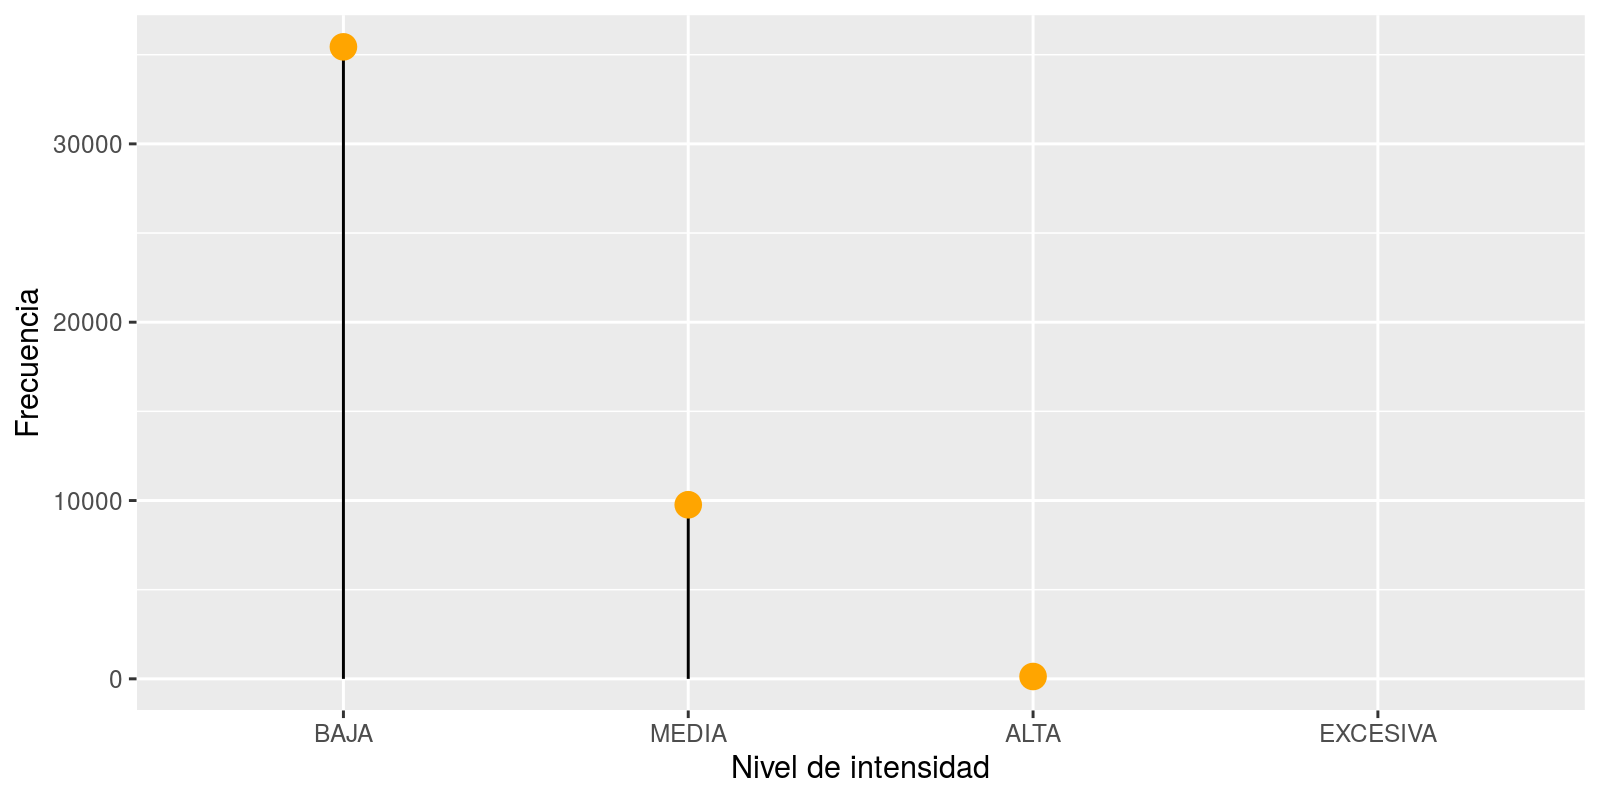
\includegraphics{./figure/unnamed-chunk-6-1} \end{center}

\begin{Shaded}
\begin{Highlighting}[]
  \KeywordTok{ggplot}\NormalTok{(Q1, }\KeywordTok{aes}\NormalTok{(}\DataTypeTok{x =} \NormalTok{carril, }\DataTypeTok{y =} \StringTok{`}\DataTypeTok{intensidad por hora}\StringTok{`}\NormalTok{, }\DataTypeTok{fill =} \NormalTok{carril)) +}\StringTok{ }
\StringTok{    }\KeywordTok{geom_violin}\NormalTok{(}\DataTypeTok{draw_quantiles =} \KeywordTok{c}\NormalTok{(}\FloatTok{0.25}\NormalTok{, }\FloatTok{0.5}\NormalTok{, }\FloatTok{0.75}\NormalTok{), }\DataTypeTok{scale =} \StringTok{"width"}\NormalTok{) +}
\StringTok{    }\KeywordTok{geom_hline}\NormalTok{(}\DataTypeTok{yintercept =} \DecValTok{2400}\NormalTok{, }\DataTypeTok{linetype =} \StringTok{"dashed"}\NormalTok{, }\DataTypeTok{color =} \StringTok{"#FF0000"}\NormalTok{, }\DataTypeTok{size =} \FloatTok{1.2}\NormalTok{) +}
\StringTok{    }\KeywordTok{theme_bw}\NormalTok{()}
\end{Highlighting}
\end{Shaded}

\begin{center}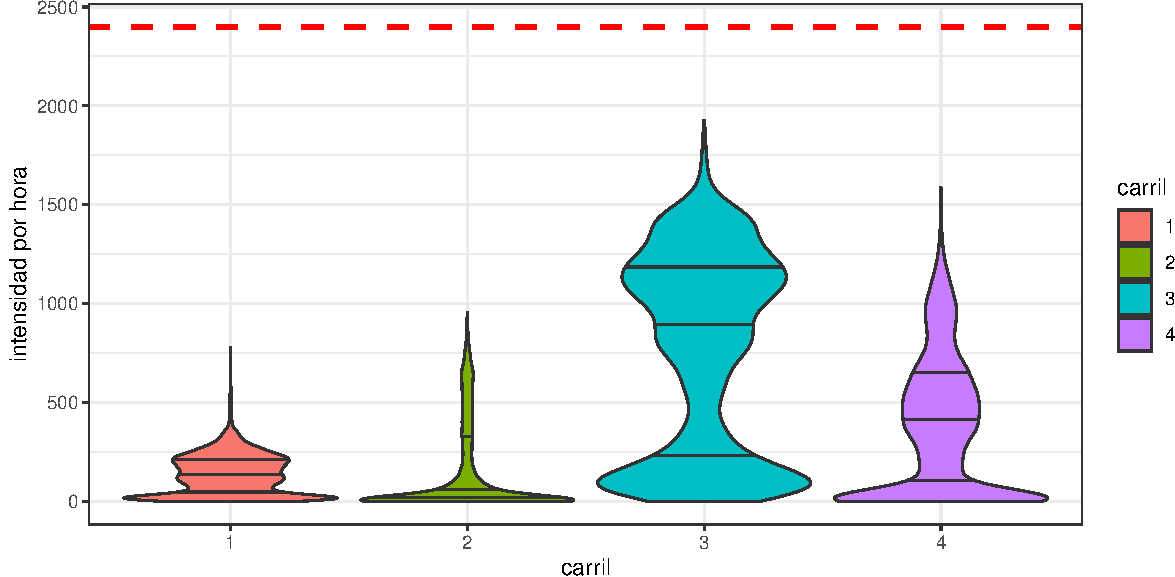
\includegraphics{./figure/unnamed-chunk-6-2} \end{center}

\begin{Shaded}
\begin{Highlighting}[]
\CommentTok{#ggplot(TD, aes(x = `velocidad media`, y = `intensidad total`)) + geom_point()}
\end{Highlighting}
\end{Shaded}

PROPUESTA: ¿En què mes hubo mayor intensidad, por carril?

\begin{Shaded}
\begin{Highlighting}[]
\NormalTok{Q2 <-}\StringTok{ }\NormalTok{TD %>%}
\StringTok{      }\KeywordTok{group_by}\NormalTok{(año, mes, carril) %>%}
\StringTok{      }\KeywordTok{summarise}\NormalTok{(}\StringTok{`}\DataTypeTok{total}\StringTok{`}   \NormalTok{=}\StringTok{ }\KeywordTok{mean}\NormalTok{(}\StringTok{`}\DataTypeTok{intensidad total}\StringTok{`}\NormalTok{),}
                \StringTok{`}\DataTypeTok{ligeros}\StringTok{`} \NormalTok{=}\StringTok{ }\KeywordTok{mean}\NormalTok{(}\StringTok{`}\DataTypeTok{intensidad ligeros}\StringTok{`}\NormalTok{)) %>%}
\StringTok{      }\KeywordTok{gather}\NormalTok{(}\DataTypeTok{key =} \StringTok{"Tipo de intensidad"}\NormalTok{, }
             \DataTypeTok{value =} \StringTok{"Intensidad"}\NormalTok{, }\StringTok{`}\DataTypeTok{total}\StringTok{`}\NormalTok{, }\StringTok{`}\DataTypeTok{ligeros}\StringTok{`}\NormalTok{)}

\KeywordTok{ggplot}\NormalTok{(Q2, }\KeywordTok{aes}\NormalTok{(}\DataTypeTok{x =} \NormalTok{mes, }\DataTypeTok{y =} \NormalTok{Intensidad, }\DataTypeTok{fill =} \StringTok{`}\DataTypeTok{Tipo de intensidad}\StringTok{`}\NormalTok{)) +}\StringTok{ }
\StringTok{      }\KeywordTok{geom_bar}\NormalTok{(}\DataTypeTok{stat =} \StringTok{"identity"}\NormalTok{, }\DataTypeTok{position =} \StringTok{"dodge"}\NormalTok{) +}
\StringTok{      }\KeywordTok{facet_wrap}\NormalTok{(}\KeywordTok{vars}\NormalTok{(año, carril), }\DataTypeTok{ncol =} \DecValTok{2}\NormalTok{,}
                 \DataTypeTok{labeller =} \StringTok{"label_both"}\NormalTok{, }\DataTypeTok{strip.position =} \StringTok{"top"}\NormalTok{) +}
\StringTok{      }\KeywordTok{ggtitle}\NormalTok{(}\StringTok{"Intensidad en tráfico mensual"}\NormalTok{) +}
\StringTok{      }\KeywordTok{xlab}\NormalTok{(}\StringTok{"Meses"}\NormalTok{) +}
\StringTok{      }\KeywordTok{ylab}\NormalTok{(}\StringTok{"Intensidad"}\NormalTok{) +}
\StringTok{      }\KeywordTok{theme_minimal}\NormalTok{() +}
\StringTok{      }\KeywordTok{theme}\NormalTok{(}\DataTypeTok{strip.text =} \KeywordTok{element_text}\NormalTok{(}\DataTypeTok{size =} \DecValTok{14}\NormalTok{),}
            \DataTypeTok{axis.text.x =} \KeywordTok{element_text}\NormalTok{(}\DataTypeTok{angle =} \DecValTok{45}\NormalTok{, }\DataTypeTok{hjust =} \DecValTok{1}\NormalTok{),}
            \DataTypeTok{legend.title =} \KeywordTok{element_blank}\NormalTok{(),}
            \DataTypeTok{axis.text =} \KeywordTok{element_text}\NormalTok{(}\DataTypeTok{size =} \DecValTok{14}\NormalTok{),}
            \DataTypeTok{axis.title =} \KeywordTok{element_text}\NormalTok{(}\DataTypeTok{size =} \DecValTok{14}\NormalTok{))}
\end{Highlighting}
\end{Shaded}

\begin{center}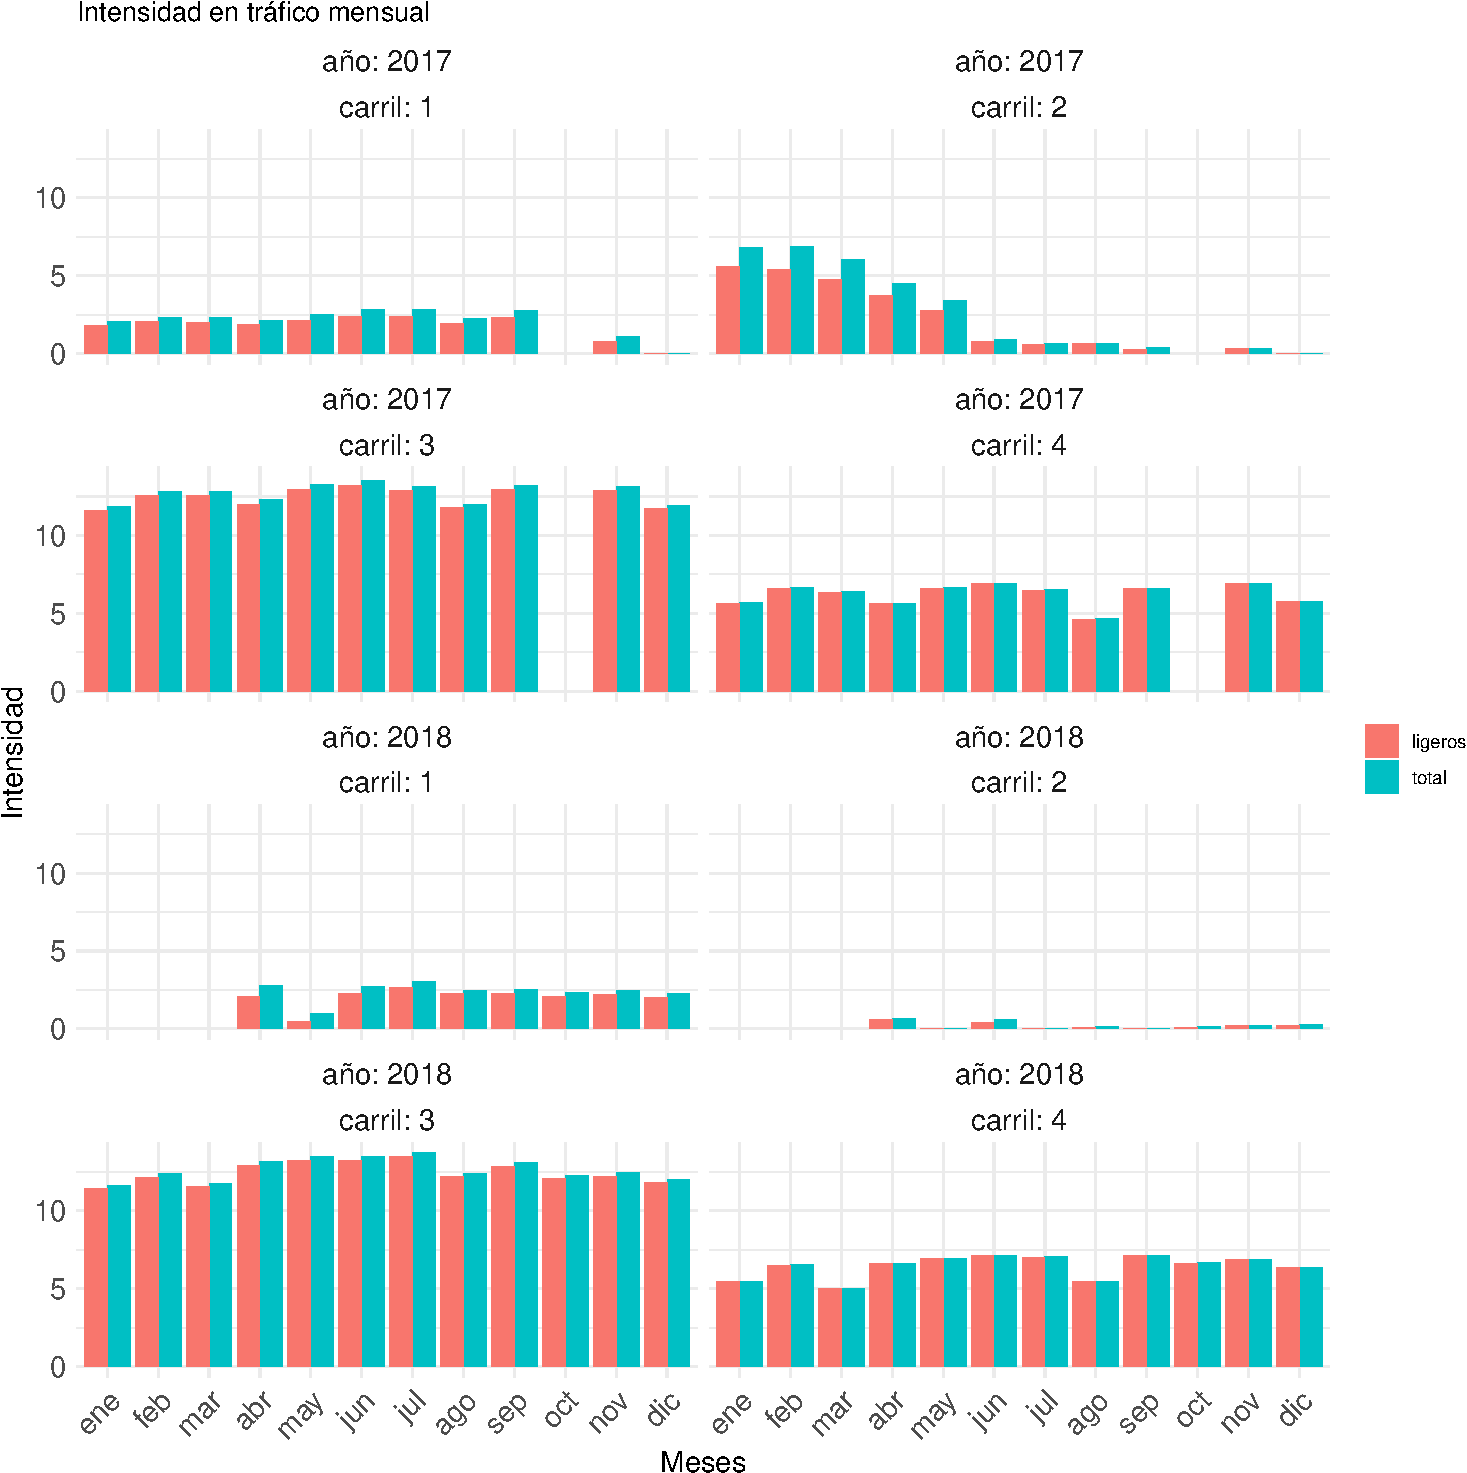
\includegraphics{./figure/unnamed-chunk-7-1} \end{center}

PROPUESTA: ¿Cómo se distribuye la intensidad, por carril y por hora-año?

\begin{Shaded}
\begin{Highlighting}[]
\NormalTok{Q3 <-}\StringTok{ }\NormalTok{TD %>%}
\StringTok{      }\KeywordTok{select}\NormalTok{(año, hora, carril, }\StringTok{`}\DataTypeTok{intensidad total}\StringTok{`}\NormalTok{) %>%}
\StringTok{      }\KeywordTok{group_by}\NormalTok{(año, hora, carril) %>%}
\StringTok{      }\KeywordTok{summarise}\NormalTok{(}\DataTypeTok{total =} \KeywordTok{mean}\NormalTok{(}\StringTok{`}\DataTypeTok{intensidad total}\StringTok{`}\NormalTok{))}

\KeywordTok{ggplot}\NormalTok{(Q3, }\KeywordTok{aes}\NormalTok{(}\DataTypeTok{x =} \NormalTok{hora, }\DataTypeTok{y =} \NormalTok{total, }\DataTypeTok{fill =} \NormalTok{carril)) +}\StringTok{ }
\StringTok{      }\KeywordTok{geom_bar}\NormalTok{(}\DataTypeTok{stat =} \StringTok{"identity"}\NormalTok{, }\DataTypeTok{position =} \StringTok{"dodge"}\NormalTok{, }\DataTypeTok{color =} \StringTok{"black"}\NormalTok{) +}
\StringTok{      }\KeywordTok{geom_smooth}\NormalTok{(}\KeywordTok{aes}\NormalTok{(}\DataTypeTok{color =} \KeywordTok{as.factor}\NormalTok{(año)),}
                \DataTypeTok{se =} \OtherTok{FALSE}\NormalTok{,}
                \DataTypeTok{lwd =} \DecValTok{1}\NormalTok{,}
                \DataTypeTok{alpha =} \FloatTok{0.5}\NormalTok{) +}
\StringTok{      }\KeywordTok{scale_fill_brewer}\NormalTok{(}\DataTypeTok{palette =} \DecValTok{15}\NormalTok{) +}
\StringTok{      }\KeywordTok{facet_wrap}\NormalTok{(}\KeywordTok{vars}\NormalTok{(año, carril), }\DataTypeTok{ncol =} \DecValTok{2}\NormalTok{,}
                 \DataTypeTok{labeller =} \StringTok{"label_both"}\NormalTok{, }\DataTypeTok{strip.position =} \StringTok{"top"}\NormalTok{, }\DataTypeTok{scale =} \StringTok{"free_y"}\NormalTok{) +}
\StringTok{      }\KeywordTok{ggtitle}\NormalTok{(}\StringTok{"Intensidad en tráfico horaria por carril"}\NormalTok{) +}
\StringTok{      }\KeywordTok{xlab}\NormalTok{(}\StringTok{"Horas"}\NormalTok{) +}
\StringTok{      }\KeywordTok{ylab}\NormalTok{(}\StringTok{"Intensidad promedio anual"}\NormalTok{) +}
\StringTok{      }\KeywordTok{theme_bw}\NormalTok{() +}
\StringTok{      }\KeywordTok{theme}\NormalTok{(}\DataTypeTok{strip.text =} \KeywordTok{element_text}\NormalTok{(}\DataTypeTok{size =} \DecValTok{14}\NormalTok{),}
            \DataTypeTok{axis.text.x =} \KeywordTok{element_text}\NormalTok{(}\DataTypeTok{angle =} \DecValTok{45}\NormalTok{, }\DataTypeTok{hjust =} \DecValTok{1}\NormalTok{),}
            \DataTypeTok{legend.title =} \KeywordTok{element_blank}\NormalTok{(),}
            \DataTypeTok{axis.text =} \KeywordTok{element_text}\NormalTok{(}\DataTypeTok{size =} \DecValTok{14}\NormalTok{),}
            \DataTypeTok{axis.title =} \KeywordTok{element_text}\NormalTok{(}\DataTypeTok{size =} \DecValTok{14}\NormalTok{))}
\end{Highlighting}
\end{Shaded}

\begin{center}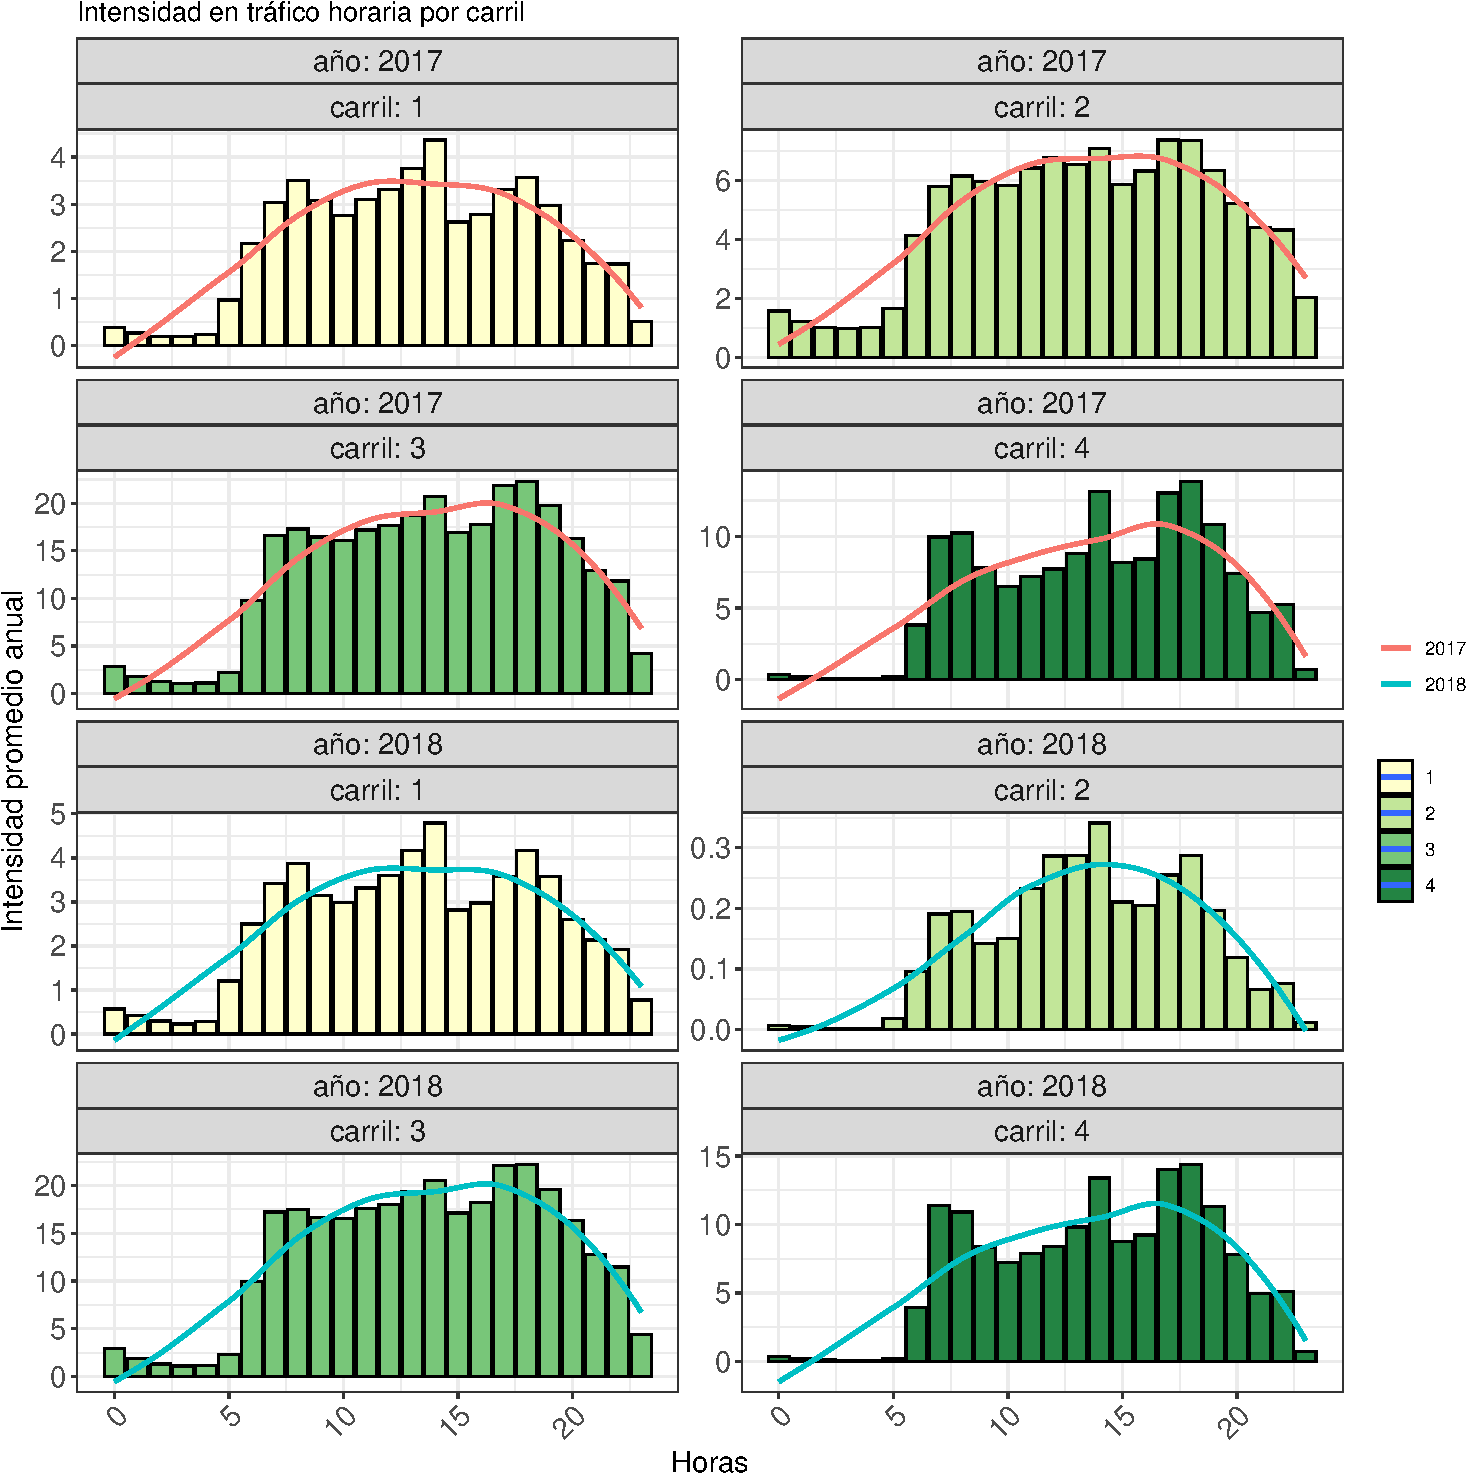
\includegraphics{./figure/unnamed-chunk-8-1} \end{center}

\begin{Shaded}
\begin{Highlighting}[]
\NormalTok{Q <-}\StringTok{ }\NormalTok{TD %>%}
\StringTok{  }\KeywordTok{select}\NormalTok{(}\StringTok{`}\DataTypeTok{intensidad total}\StringTok{`}\NormalTok{:}\StringTok{`}\DataTypeTok{distancia media entre vehiculos}\StringTok{`}\NormalTok{) %>%}
\StringTok{  }\KeywordTok{filter_all}\NormalTok{(}\KeywordTok{all_vars}\NormalTok{(. !=}\StringTok{ }\DecValTok{0}\NormalTok{))}

\CommentTok{#ggpairs(Q)}
\end{Highlighting}
\end{Shaded}

Correlación\ldots{}


\end{document}
